\documentclass{beamer}
%
% Choose how your presentation looks.
%
% For more themes, color themes and font themes, see:
% http://deic.uab.es/~iblanes/beamer_gallery/index_by_theme.html
%
\mode<presentation>
{
  \usetheme{Marburg}      % or try Darmstadt, Madrid, Warsaw, ...
  \usecolortheme{sidebartab} % or try albatross, beaver, crane, ...
  \usefonttheme{structuresmallcapsserif}  % or try serif, structurebold, ...
  \setbeamertemplate{navigation symbols}{}
  \setbeamertemplate{caption}[numbered]
} 

\usepackage[english]{babel}
\usepackage[utf8x]{inputenc}
\usepackage{graphicx, array, tabularx}

\newcommand{\mycal}{\href{http://www.nextproject.ca/seek/calendar}{bit.ly/asyeb}}

\title[Get to Know SEEK]{Get to Know SEEK\\}
\author{Ahmad Touseef\inst{1}}
\institute{\inst{1}Executive Team of SEEK\\Software \& Electrical Engineering Klub\\
Campus Clubs at Student Association of DC \& UOIT\\
\texttt{\href{mailto:team@seekuoitdc.com}{team@seekuoitdc.com}}
}
\date{\today}

\begin{document}

\begin{frame}
  \titlepage
\end{frame}

% Uncomment these lines for an automatically generated outline.
%\begin{frame}{Outline}
%  \tableofcontents
%\end{frame}

\section{About Us}

\begin{frame}{What We Do}

\begin{itemize}
\item A technical club managed by students
\item Funded by Student Association at DC \& UOIT
\item Gives practical engineering experience
\item Gives free access of parts to prototype electronics
\item Gives free access of real world software projects
\end{itemize}
\vskip 1cm
\begin{block}{You Take Away}
Real world engineering experience at SEEK. Take credit for engineering design projects you complete. Develop the skills employers need before Co-Op or Intern-Ships.
\end{block}

\end{frame}

\subsection{Big Picture}

\begin{frame}{How We Work}

\begin{figure}
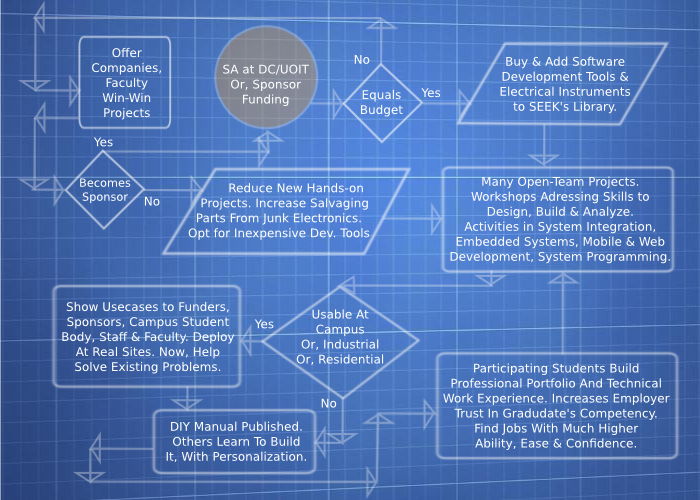
\includegraphics[scale=0.45]{howwework}
\caption{Flow chart of how SEEK operate as club}
\end{figure}

\end{frame}

\begin{frame}{Why Important}
It takes practical skills to build and re-make. Technology, Math and Science courses teach theory and applications on paper. SEEK gives you technical consulting and resources to make your theory knowledge and creative passion into solutions and products. All for free. Period.
\vskip 0.3cm
\begin{itemize}

\item Learn/use skills to engineer real world products
\item Publish your projects at blogs, academic or industry or campus peer reviewd journals, conferences
\item Use LGPL\textsuperscript{1} to license your prototypes, products
\end{itemize}
\vskip 0.3cm \textsuperscript{1}Lesser GNU Public License. Easy explanation on slide~\pageref{LGPL}. 
\end{frame}

\subsection{Execs}

\begin{frame}
\frametitle{Who Are Current Execs}
Executives are elected club members who put extra volunteer hours in any of the club positions on slide~\pageref{StudentExec}.
\begin{center}
\begin{figure}
\begin{tabular}{c c c c}
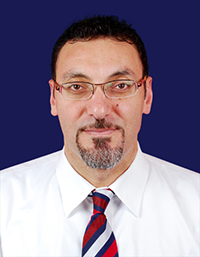
\includegraphics[scale=0.2]{QusayMahmoud} & 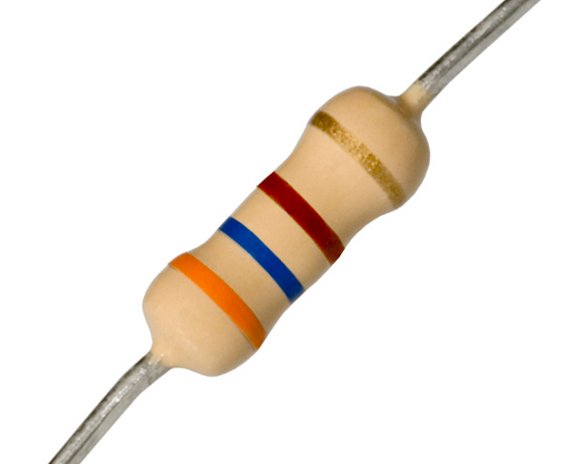
\includegraphics[scale=0.09]{resistor} & 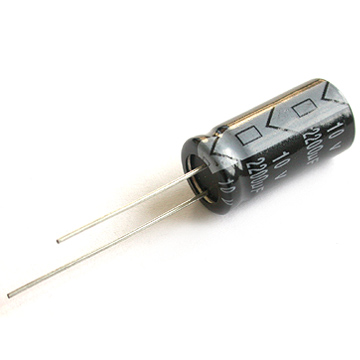
\includegraphics[scale=0.12]{capacitor} & 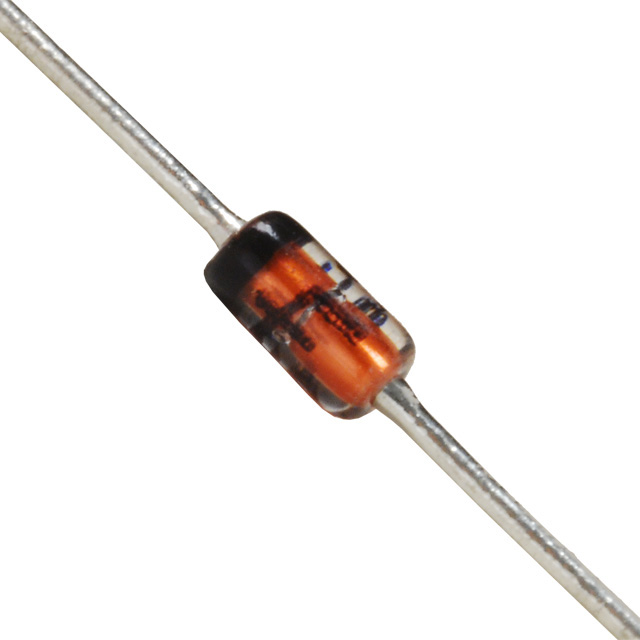
\includegraphics[scale=0.08]{diode}\\
a. & b. & c. & d.\\

\includegraphics[scale=0.6]{transistor} & 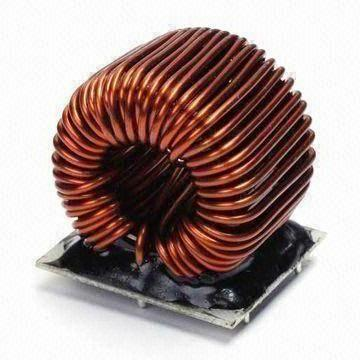
\includegraphics[scale=0.12]{inductor} & 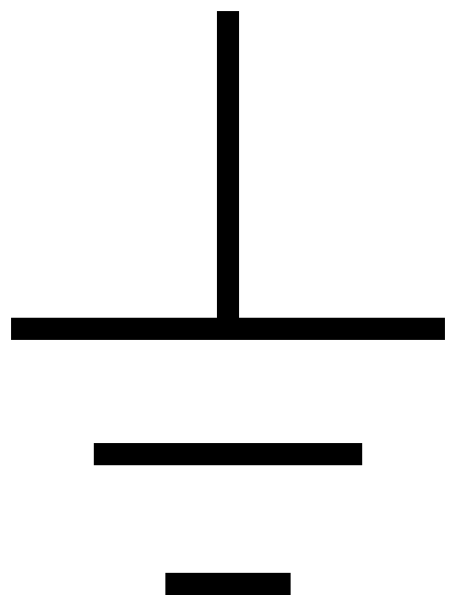
\includegraphics[scale=2.6]{ground} & \\
e. & f. & g. &\\
\end{tabular}
\caption{SEEK's 2014 executive team consisted of (a) Prof. Qusay Mahmoud (b) Michael Lescisin (c) Ahmad Touseef (d) Dhimiter Qendri (e) Shreyasi Panda (f) Paul Azevedo (g) Sagar Desai}
\end{figure}
\end{center}
\end{frame}

\subsection{Partners}

\begin{frame}
\frametitle{Campus Partners}
Ensure SEEK can maximize its resources and broaden scope of projects for students.
\begin{figure}
\begin{tabular}{c c c c}

\includegraphics[scale=0.35]{salogo} & 
\includegraphics[scale=0.22]{ieeeuoitlogo} & 
\includegraphics[scale=0.1]{csclublogo} & 
\includegraphics[scale=0.1]{nextprojectlogo}\\
\tiny a. & \tiny b. & \tiny c. & \tiny d.\\

\includegraphics[scale=0.27]{uoitengsoclogo} & & &\\
\tiny e.\\
\end{tabular}
\caption{\tiny(a) Campus Clubs of SA is primary funder for SEEK (b) McNaughton Center of IEEE Student Chapter shares their electronics prototyping tools \& parts that are not duplicated with SEEK's parts library (c) CS-Club has led the example for SEEK of open source and rapid prototyping of software products on campus (d) Dept. of ECSE outreach "NextProject" guides SEEK to realize what technical themes \& products are growing relevant to current consumers and industries (e) UOIT Engineering Student Society sponsors and funds competitions for SEEK}
\end{figure}
\end{frame}

\begin{frame}
\frametitle{Knowledge Partners}
Enable SEEK to have learning access to free or reduced price use of tool sets and technologies.
\begin{figure}
\begin{tabular}{c c}

\includegraphics[scale=0.3]{microsoftstudentpartnerlogo} & 
\includegraphics[scale=0.15]{linuxfoundationlogo}\\
\tiny a. & \tiny b.
\end{tabular}
\caption{\tiny (a) Microsoft sponsors mobile development workshops at SEEK (b) Linux Foundation gives free training course material in Open Source, Embedded and Distributed System Software Projects}
\end{figure}
\end{frame}

\section{Events}

\begin{frame}

\frametitle{Attend Club Events}

\begin{itemize}
  \item See real world demos of software \& electronic products designed \& engineered by student effort
  \item No nonsense prototyping skills delivered to you
  \item Use for free all club equipment, hardware \& tools library to make your ideas functional products
  \item Get on-demand help from club execs and interns
  \item Meet student experts in operating, embedded, control, telecommunications systems, compilers, artificial intelligence, data mining, software languages and hardware design, computer \& physical sciences, micro electronics, signal processing, analog \& power systems
\end{itemize}

\vskip 0.5cm

\begin{block}{Reminder}
\textbf{\textit{Don't miss event, view {Calendar} at \mycal}}
\end{block}

\end{frame}

\begin{frame}
\frametitle{Build Parties}
\begin{itemize}
\item Get free loan out of parts \& tools
\item Get free expert help on building hardware \& software
\item Build electronics and computers from scratch
\item Develop programs solving real world problems
\item Test and deploy your products to masses
\item Learn important industry practices \& standards in EE \& SE design engineering through practice
\item Learn by doing (often overlooked) prototyping, repair, problem diagnosis \& troubleshooting skills
\end{itemize}
\end{frame}

\begin{frame}
\frametitle{Workshops}
\begin{itemize}
\item Gives you live demo of student built projects
\item Teaches you how to create electronics you use everyday
\item Get free help in solving your questions and challenges
\end{itemize}
\end{frame}

\begin{frame}
\frametitle {Distance Learning}
\begin{itemize}
\item Read workshops on line, after they finish via links in SEEK's calendar itself at \mycal
\item Workshops will introduce you to practical engineering topics, where as build parties will 
\item Learn prototyping skills used by EE \& SE experts
\end{itemize}
\end{frame}

\begin{frame}
\frametitle {Competitions}
\begin{itemize}
\item Are implemented by SEEK and sponsored by partners
\end{itemize}
\end{frame}

\subsection{When}

\begin{frame}{When Events Held}
\begin{itemize}
\item Help and tutorials on Thursdays
\item Build "parties" \& Maker events on Mondays, Fridays
\item Starts at \textbf{11:00am}
\item Flexible when ends; just show up within first hour
\vskip 1cm
\begin{block}{Don't Forget}
\textbf{Calendar} shows all planned events. View it at \mycal
\end{block}
\end{itemize}
\end{frame}

\subsection{Where}
\begin{frame}{Where Are We}

\begin{itemize}
\item Share office at room ACE 4030\textsuperscript{1} with IEEE McNaghton Center
\item Hold hands-on, maker events at J 127\textsuperscript{2}
\item Competitions happen at GW 210\textsuperscript{3}
\item Parts \& prototyping tools library stored at SA Club Lockers in UL 1020\textsuperscript{4}
\end{itemize}
\vskip 1cm
\textsuperscript{1}Automotive Center of Excellence Bldg.
\textsuperscript{2}J Wing of Simcoe Bldg.
\textsuperscript{3}Gordon Wiley Bldg.
\textsuperscript{4}UL Student Portables\\[10pt]
\hfill
\end{frame}

\section{Contribute As}

\begin{frame}{Benefits}

\begin{block}{For Students}
\begin{itemize}
\item Get credits on official transcript
\item Get recognition by completing club extracurricular jobs or contributing to club projects
\end{itemize}
\end{block}

\begin{block}{Industry}
\begin{itemize}
\item Get free use cases and demo for your products
\end{itemize}
Technical student experts use your sponsored tools and equipment to research, experiment and produce documented and videoed tutorials on using your products. Tutorials and guides for your products are produced for you for free.
\end{block}

\end{frame}

\subsection{Student Exec}

\begin{frame}[label={StudentExec}]
\frametitle{Student Exec}

You choose a position and campaign for it. SEEK members' vote elects you to take that position. As exec you get real technical and leadership experience.

\begin{table}[ht]
\tiny
\begin{tabular}{>{\centering\arraybackslash\bfseries}m{1in} >{\centering\arraybackslash}m{6.8cm}}
President & Decides purchase of new hardware via "purchase form". Signs out equipment via "signout form". Gives extra help to beginners. \\
Vice President & Gets new sponsors to hold competitions and issue projects. Assists other executives to stay up do speed. Prepares supplementary applications.\\
Chief Auditor General & Ensures equipment in "current inventory" match equipment in SEEK lockers. Prevents loss and theft of items. Acquires fines for late returns.\\
VP Embedded Systems & Teaches and does demo on making instruments, gadgets, communication and network devices. Suggests new purchases for "future equipment".\\
VP Server Systems & Maintains mirrors for popular Open Source software package repositories. Teaches about cluster, parallel \& distributed computing, mesh networking\\
VP Electric Machines & Teaches and demo on electric motor, generator and energy devices. Observes trends in market and initiates relevant projects.\\
VP Mobile Systems & Teaches ad does demo on iOS, Android and Blackberry programming. Observes mobile app trends and initiates relevant development projects. \\
VP Client Programming & Teaches and does demo web browser client programming. Observes web browser trends and initiates relevant development projects for club.
\end{tabular}
\caption{SEEK student executive positions and descriptions}
\end{table}
\end{frame}

\subsection{Hardware Sponsor}

\begin{frame}{Hardware Sponsor Benefits}
\begin{itemize}
\item We develop and document use cases for you
\item We create teaching material with demos with your hardware
\item Benefit from lowering the learning gap of users of your products
\item Integrate our tutorials and projects with your hardware on your business website, blogs and show case media to reveal the highest potential of your products
\item Benefit from student technical talent with proven expertise, at no cost
\end{itemize}
\end{frame}

\subsection{Software Sponsor}

\begin{frame}{Software Sponsor Benefits}
\begin{itemize}
\item We develop and document use cases for you
\item We create teaching material with demos with your hardware
\item Benefit from lowering the learning gap of users of your products
\item Integrate our tutorials and projects with your hardware on your business website, blogs and show case media to reveal the highest potential of your products
\item Benefit from student technical talent with proven expertise, at no cost
\end{itemize}
\end{frame}

\subsection{Faculty Mentor}

\begin{frame}{Faculty Mentor Benefits}

Every week give an hour of consulting to the club. Inspire highly motivated students to initiate projects that you are unable to. Network with campus, undiscovered maker community, whose work may help you find best research assistants on campus.

\end{frame}

\section{FAQ}

\subsection{Lgpl}

\begin{frame}[label={LGPL}]
\frametitle{Is LGPL for Me?}

E-mail \texttt{\href{mailto:michael.lescisin@uoit.net}{michael.lescisin@uoit.net}} to discuss if LGPL suits your projects. If it is unsuitable, she will help you decide on best license for your inventions, projects and products.

\end{frame}

\subsection{Transcript Rec.}

\begin{frame}{Show Involvement on Official Transcript}
Submit application at Student Experience UOIT in March 2015 to get involvement credits in your official transcript.
\end{frame}

\section{Credits}
\begin{frame}
\frametitle{Who and When Presents}
Gratitude to people who used these slides to present at events.
\begin{table}
\tiny
\centering
\begin{tabular}{|p{2cm}|p{2cm}|p{2.4cm}|p{1.6cm}|}
\hline
\textbf{Presenter Name} & \textbf{Date Presented} & \textbf{Event or Occasion} & \textbf{Place}\\
\hline
Sagar, Paul & Sep. 4th 2014 & Get Involved Fair & Dec \& UOIT\\
\hline
Michael Lescisin & Mon. 8\textsuperscript{th} Sep. 8th 2014 & Boot Camp & DC \& UOIT\\
\hline
\end{tabular}
\end{table}
\end{frame}

\end{document}
